    \subsection{Main функция}

    \begin{verbatim}
        undefined4 main(void)

        {
          char *pcVar1;
          int iVar2;
          undefined4 local_10;

          puts("############################################ ################");
          puts("##        Bienvennue dans ce challenge de cracking        ##" );
          puts("############################################ ################\n");
          printf("username: ");
          pcVar1 = (char *)getString(local_10);
          iVar2 = strcmp(pcVar1,"john");
          if (iVar2 == 0) {
             printf("password: ");
             pcVar1 = (char *)getString(pcVar1);
             iVar2 = strcmp(pcVar1,"the ripper");
             if (iVar2 == 0) {
                printf("Bien joue, vous pouvez valider l'epreuve avec le mot d e passe : %s !\n","987654321");
             }
             else {
                puts("Bad password");
             }
          }
          else {
             puts("Bad username");
          }
          return 0;
        }
    \end{verbatim}

    \subsection{Описание}

    Программа реализует простую аутентификационную логику.
    Пользователю предлагается ввести имя пользователя и пароль.
    Проверка осуществляется путём прямого сравнения введённых строк с жёстко заданными значениями.

    \begin{itemize}
        \item Если имя пользователя совпадает с \texttt{"john"}, то далее проверяется пароль.
        \item Если пароль совпадает с \texttt{"the ripper"}, то выводится сообщение об успехе и секретный ключ.
        \item В противном случае программа сообщает об ошибке (\texttt{"Bad username"} или \texttt{"Bad password"}).
    \end{itemize}

    \subsection*{Ключ (флаг)}

    Если логин и пароль указаны верно, программа выводит:

    \begin{verbatim}
        Bien joue, vous pouvez valider l'epreuve avec le mot de passe : 987654321 !
    \end{verbatim}


    \subsection{Особенности}

    \begin{itemize}
        \item Логика крайне простая — всё полностью зашито в бинарник.
        \item Пароли не шифруются, не хэшируются и не скрыты — можно легко найти через \texttt{strings} или дизассемблирование.
        \item Юзернейм - "john", пароль - "the ripper"
        \item Ключ - 987654321
    \end{itemize}

    \subsection{Тестовые запуски}
    \paragraph{}
    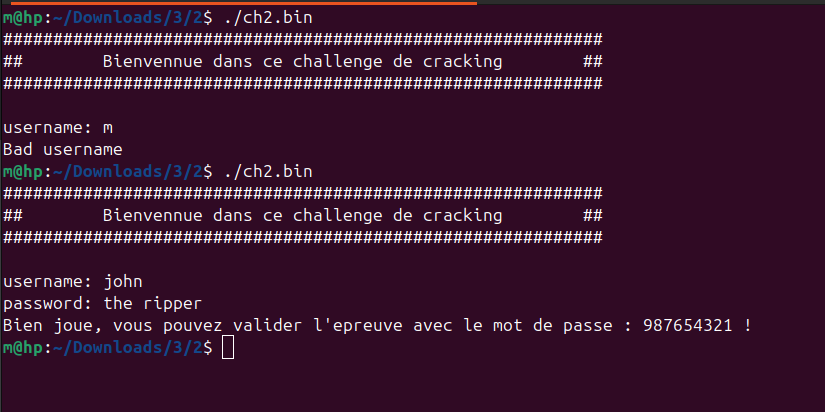
\includegraphics[width=1\linewidth]{static/solution_2}
